\documentclass{article}
\usepackage{amsmath}
\usepackage{amssymb}
\usepackage{algorithm}
\usepackage{float}
\usepackage{color}
\usepackage{multicol}

\usepackage{graphicx}
\graphicspath{ {./} }
\title{Neural Networks Final Project: \\
	\large{Comparing different data pre-processing techniques for convolution neural networks}}
\author{Krystian Wojcicki, 101001444 \\ Michael Kuang, 101000485}
\date{COMP 4107, Fall 2018}

\begin{document}
\maketitle

\newpage

\section{Introduction}
\paragraph{}
{\em Natural Images} is a dataset currently featured on {\em kaggle.com}. The set is comprised of 6899 images from 8 distinct classes of airplane, car, cat, dog, flower, fruit, motorbike and person. Each class has a varying number of examples. We examined different techniques in pre-processing images and implemented them to analyze their effects on performance in a convolution neural network. 

\section{Problem Statement}
\paragraph{}
This project attempts to address the problems: "Do different image resizing techniques make a difference to classification accuracy?" and "Do balanced datasets improve classification accuracy?".

\section{Background}
\paragraph{}
One problem we looked at is the Class Imbalance problem, and this is the problem in machine learning where we have great discrepancy in the number of examples between class data. In other words, there are far more examples of one class than another in a set of data. This is a problem because as we know, machine learning works best when we have a more uniform distribution of data. In this project, we examine the performance between two up-sampling techniques called SMOTE and ADASYN as solutions to class imbalance. 
\par
Another problem we investigated is how image resizing can affect performance. Given a set of non-uniform sizes of images, we must resize them to some constant shape in order to feed examples into the network. We examined two methods; resize the image by scaling it, and crop or pad the image about the center. The problem with resizing an image is that we inevitably lose information as images are scaled down or add noise as they are scaled up. Cropping the image will directly lose the information as we resize the image by cropping out the outer most part of the image, while padding the image with black pixels evenly about center will retain the image aspect ratio.

\subsection{The Dataset}
\paragraph{}
The {\em Natural Images} dataset contains 6899 distinct RGB images of varying sizes for 8 classes as described below:
\begin{multicols}{2}

\begin{itemize}
	\item airplane: 727 
	\item car: 968
	\item cat: 885
	\item dog: 702
	\item flower: 843
	\item fruit: 1000
	\item motorbike: 788
	\item person: 986
\end{itemize} 

\end{multicols}
\subsection{Machine Learning Libraries}
\paragraph{}
Four libraries were used to implement our code, and create our neural network model: Tensorflow, scikit-learn, imbalanced-learn and OpenCV.

\subsection{Methodology}

\subsubsection{Scaling vs Crop and Pad}
\paragraph{}
We used OpenCV's resize method to scale the images down to or up to a specified size using nearest neighbour interpolation. The nearest neighbour interpolation is a point sampling algorithm that, rather than calculate the average or some weighting criteria, simply determines the nearest neighbouring pixel and assumes the intensity value of it. Using this method, it will upscale or downscale to a specified size. This method will add noise when we upscale or lose information when we downscale, and it is noted that the image will lose its original aspect ratio.
\par
Resizing an image by crop and pad means that the image will retain it's image resolution, but we either crop or pad the image about the center to the specified size. So, if the height of the image needs to be smaller, we crop the top and bottom evenly. Conversely, if the height of the image needs to be larger, we evenly pad the top and bottom with black pixels.	

To crop images, we simply used Python's built in array slicing on numpy arrays. Then, to pad or resize images, we used the following methods from the OpenCV library:
\begin{itemize}
	\item cv2.copyMakeBorder: padded the borders of the image by a specified amount using pixel color value of 0
	\item cv2.resize: resizes a given image to a specified height and width using interpolation method INTER\_NEAREST
\end{itemize}

\subsubsection{Over-sampling vs Under-sampling}
\paragraph{}
Over-sampling balances a dataset by randomly duplicating the "better" representations of elements from the minority classes. However, this may cause over fitting because of the duplications. Under-sampling balances a dataset by randomly eliminating elements uniformly from the majority classes as it makes a K-means to reduce the number of samples. 

To over- and under-sample our dataset, we used the following methods from the imbalance-learn library:

\begin{itemize}
	\item imblearn.over\_sampling.SMOTE: over-sampled on the image dataset using "not majority" for the \textit{sample\_strategy} parameter
	
	\item imblearn.over\_sampling.ADASYN: over-sampled on the image dataset using "not majority" for the \textit{sample\_strategy} parameter
	
\end{itemize}



\section{Results}

\section{Analysis}

\section{Discussion}

\section{Conclusion	}

\section{References	}

\section{Spatial Pyramid Pooling}

CNNs require a fixed input image size such as 32x32, 64x64 or 128x128 as experimented with in this report. This requirement is human made and artificial while also potentially decreasing recognition accuracy due to loss of content while padding or distortion while resizing. The need to fixed size inputs is due to the fully-connected layer portion of a CNN, the convolution layers use a sliding window and operate correctly on any size input. However the fully-connected portion requires a fixed-size input. To get around this Kaiming et al [2015] introduced spatial pyyramid pooling (SPP), this pooling layer is added on top of the final convolution layer and generates fixed-length outputs regardless of the size of the feature maps given to it.  \\

SPP builds on and improves the concept of Bag-of-Words (BoW), it does so but maintaining spatial information by pooling in local spatial bins. These spatial bins have sizes that are proportional to the image size meaning that the number of bins is fixed regardless of the image size.

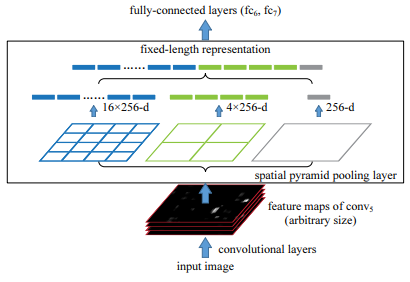
\includegraphics{spp}

For training and testing a model with an SPP layer several approaches can be taken. We chose to investigate a multi-size training approach, here we create two fixed-size networks that share parameters. Then for training we alternated by providing the network 32x32 images for one epoch and then 64x64 epochs for the next epoch. 

\end{document} 